
\subsection{Rejestracja konta użytkownika}
Funkcjonalność umożliwiająca rejestrację w aplikacji.

\subsubsection{Backend}
Po wysłaniu requesta na przez aplikacje webową lub mobilną api wyciąga przesłane dane, weryfikuje je. Do weryfikacji należy:

\begin{itemize}
    \item Czy użytkownik z wprowadzonym email istnieje już w bazie
    \item Czy użytkownik z wprowadzoną nazwą użytkownika istnieje już w bazie
    \item Czy przesłane hasła są równe
\end{itemize}

W przypadku błędnej weryfikacji zwraca odpowiednią wiadomość z błędem dla użytkownika np. “Wprowadzony email jest już zajęty”. Natomiast jeśli weryfikacja przebiegnie pomyślnie, użytkownik zostanie dodany do bazy, a system wyśle mu wiadomość email z prośbą o aktywację konta.

\begin{figure}[H]
    \centering
    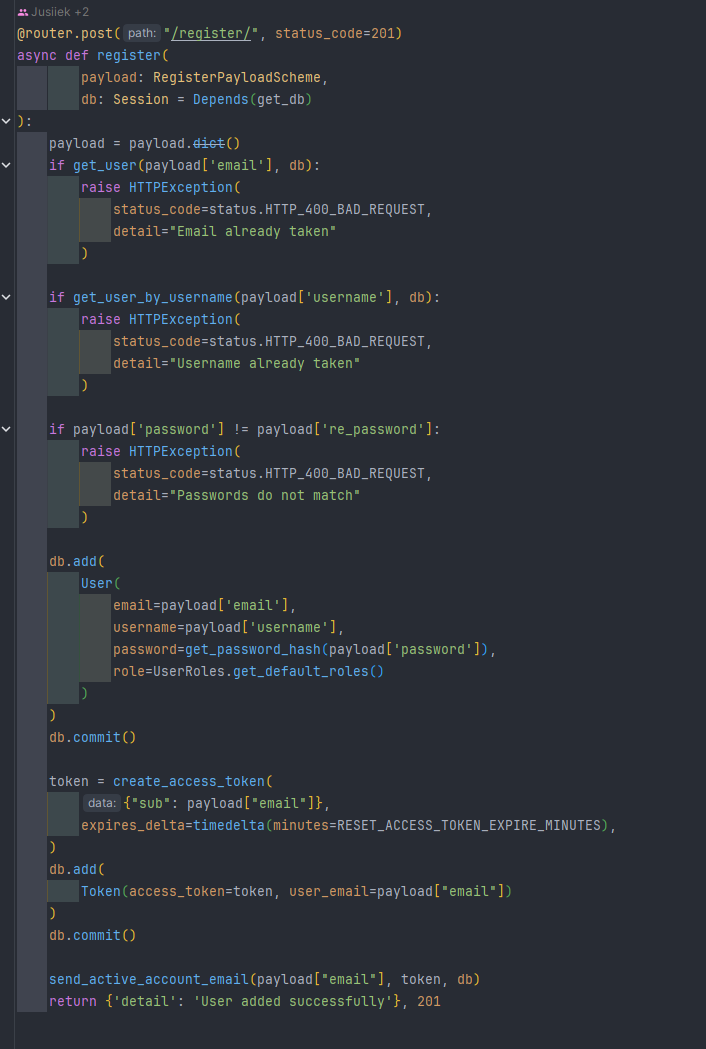
\includegraphics[width=0.7\textwidth]{chapters/chapter_8/screens/rejestracja_backend}
    \caption{Implementacja kodu rejestracji użytkownika w backendzie.}
    \label{img:rejestracja_backend}
\end{figure}

\subsubsection{Aplikacja moblina i aplikacja webowa}
Aby założyć konto, użytkownik musi wypełnić formularz rejestracyjny wymagający podania nazwy użytkownika, adresu email oraz hasła wpisanego jednakowego do dwóch pól w celach jego walidacji. Aplikacja pozwoli na utworzenie konta jedynie jeżeli:

\begin{itemize}
    \item Pseudonim zawiera od 3 do 20 znaków i składa się wyłącznie z liter, cyfr, lub podkreślników
    \item Adres e-mail jest dostarczony w prawidłowym dla niego formacie
    \item Hasło posiada co najmniej 8 znaków
    \item Hasło wpisane oba pola walidacyjne jest w nich takie samo
    \item Adres e-mail i nazwa użytkownika są unikalne (czyli w bazie danych nie są przypisane do żadnego innego konta)
\end{itemize}

Po zatwierdzeniu prawidłowych danych aplikacja informuje komunikatem o udanym utworzeniu konta. Użytkownik zostaje przeniesiony do strony logowania. W przypadku podania nieprawidłowych danych, użytkownik nie zostanie zarejestrowany i zostanie powiadomiony komunikatem w aplikacji o błędzie.

\begin{figure}[H]
    \centering
    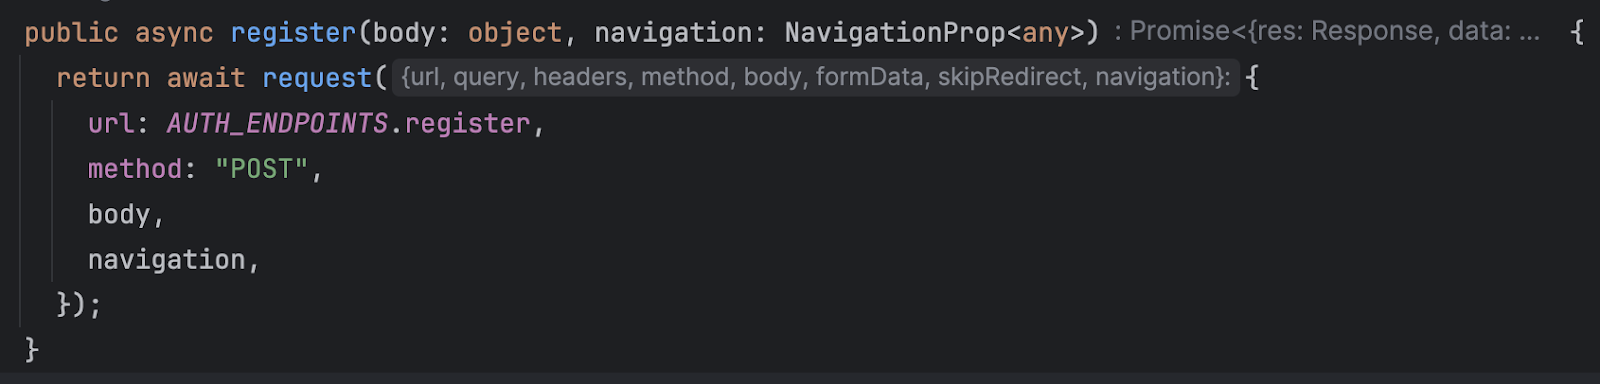
\includegraphics[width=0.7\textwidth]{chapters/chapter_8/screens/rejestracja_mobile}
    \caption{Metoda “register” w serwisie Auth zastosowana w aplikacji mobilnej.}
    \label{img:rejestracja_mobile}
\end{figure}

\begin{figure}[H]
    \centering
    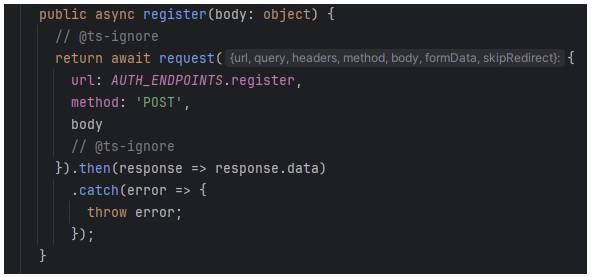
\includegraphics[width=0.7\textwidth]{chapters/chapter_8/screens/rejestracja_web}
    \caption{Metoda “register” w serwisie AuthService zastosowana w aplikacji webowej.}
    \label{img:rejestracja_web}
\end{figure}

Powyższe funkcję wysyłają asynchroniczne żądanie POST do serwera w celu rejestracji nowego użytkownika. Metoda przekazuje dane rejestracyjne w treści żądania, a następnie zwraca czy żądanie zostało obsłużone.

\subsection{Logowanie do systemu}
Funkcjonalność umożliwiająca logowanie do aplikacji

\subsubsection{Backend}
Po wysłaniu requesta na przez aplikację webową lub mobilną api wyciąga przesłane dane, weryfikuje je.
Weryfikacja odbywa się za pomocą funkcji \texttt{authenticate\_user} zaimportowaną z utils’ów.
Ta najpierw próbuje wyciągnąć z użytkownika z bazy, który posiada wysłany e-mail. Potem, jeżeli użytkownik istnieje, sprawdzamy hasło metodą klasową \texttt{verify\_password}. Jeśli wszystko przebiegło pomyślnie, użytkownikowi zostanie zwrócony token autoryzacji i dane użytkownika. W przeciwnym razie zwrócona wiadomość i błędnie wprowadzonych danych.

\begin{figure}[H]
    \centering
    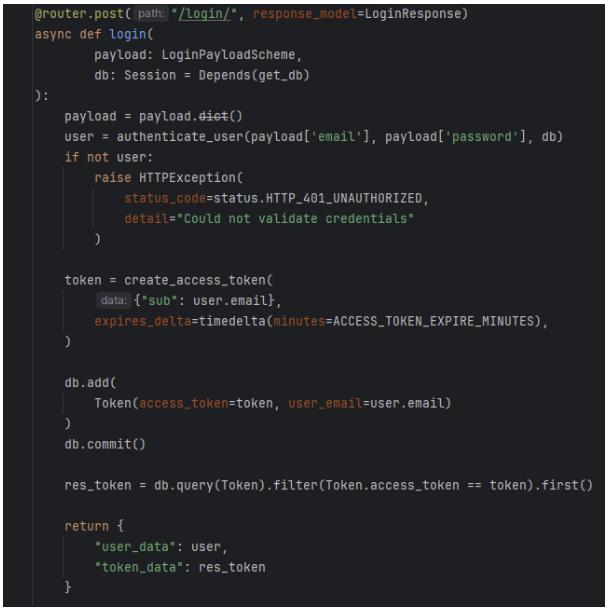
\includegraphics[width=0.7\textwidth]{chapters/chapter_8/screens/logowanie_backend}
    \caption{Implementacja kodu logowania użytkownika w backendzie.}
    \label{img:logowanie_backend}
\end{figure}

\subsubsection{Aplikacja mobilna i aplikacja webowa}
Na stronie logowania, użytkownik musi wypełnić formularz wymagający uzupełnienia pól adres email oraz hasło. Po zatwierdzeniu danych i ich weryfikacji pojawia się komunikat o zalogowaniu użytkownika, a następnie użytkownik zostanie przeniesiony na stronę główną. W przypadku podania nieprawidłowych danych, użytkownik nie zostanie zalogowany i zostanie poinformowany komunikatem o błędzie.

\begin{figure}[H]
    \centering
    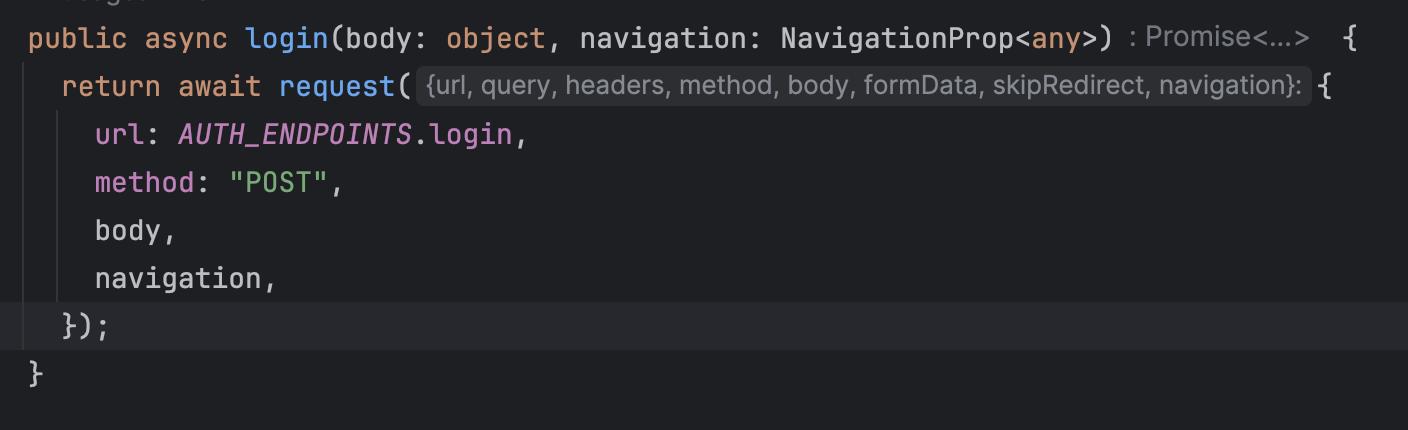
\includegraphics[width=0.7\textwidth]{chapters/chapter_8/screens/logowanie_mobile}
    \caption{Metoda “login” zastosowana w aplikacji mobilnej.}
    \label{img:logowanie_mobile}
\end{figure}

\begin{figure}[H]
    \centering
    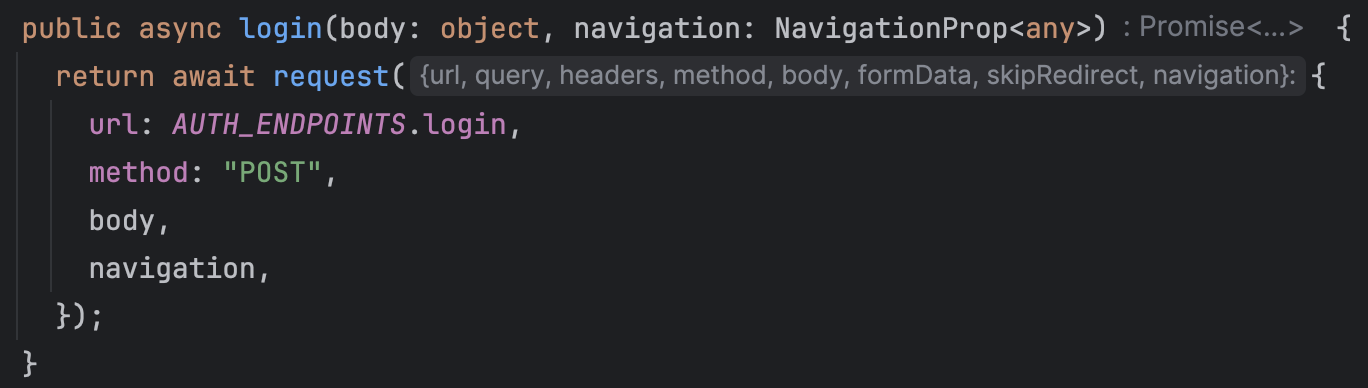
\includegraphics[width=0.7\textwidth]{chapters/chapter_8/screens/logowanie_web}
    \caption{Metoda “login” zastosowana w aplikacji webowej.}
    \label{img:logowanie_web}
\end{figure}

Użyta w powyższych metodach funkcja \texttt{ActiveUser.set(data)} zapisuje dane zalogowanego użytkownika w lokalnym stanie aplikacji. Dzięki temu, informacje o użytkowniku, takie jak token autoryzacyjny, mogą być łatwo dostępne w całej aplikacji. Pozwala to na:

\begin{itemize}
    \item Personalizację interfejsu użytkownika (np. wyświetlanie nazwy użytkownika)
    \item Umożliwienie dostępu do zasobów, które wymagają uwierzytelnienia
    \item Przechowywanie sesji użytkownika, aby mógł pozostać zalogowany pomiędzy różnymi wizytami na stronie
\end{itemize}

\subsection{Wylogowanie z systemu}
Funkcjonalność pozwalająca na wylogowanie użytkownika.

\subsubsection{Backend}
Po kliknięciu wyloguj w aplikacji mobilnej czy w webowej, zostaje wysłany request na api, który dodaje aktualnie używany token do listy nieaktualnych tokenów.

\begin{figure}[H]
    \centering
    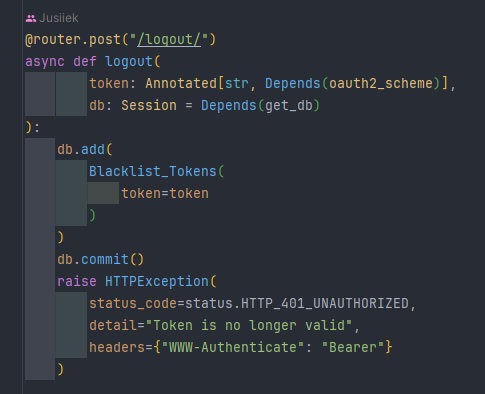
\includegraphics[width=0.7\textwidth]{chapters/chapter_8/screens/wylogowanie_backend}
    \caption{Implementacja kodu wylogowania użytkownika w backendzie.}
    \label{img:wylogowanie_backend}
\end{figure}

\subsubsection{Aplikacja mobilna i aplikacja webowa}
Aby wylogować się z aplikacji, użytkownik musi kliknąć w nawigacji logout. Po kliknięciu przycisku, dane użytkownika zostaną usunięte z pamięci lokalnej. Token autoryzacyjny użytkownika utworzony przy logowaniu zostanie dodany w bazie danych do tabeli zawierającej nieaktywne tokeny.

\begin{figure}[H]
    \centering
    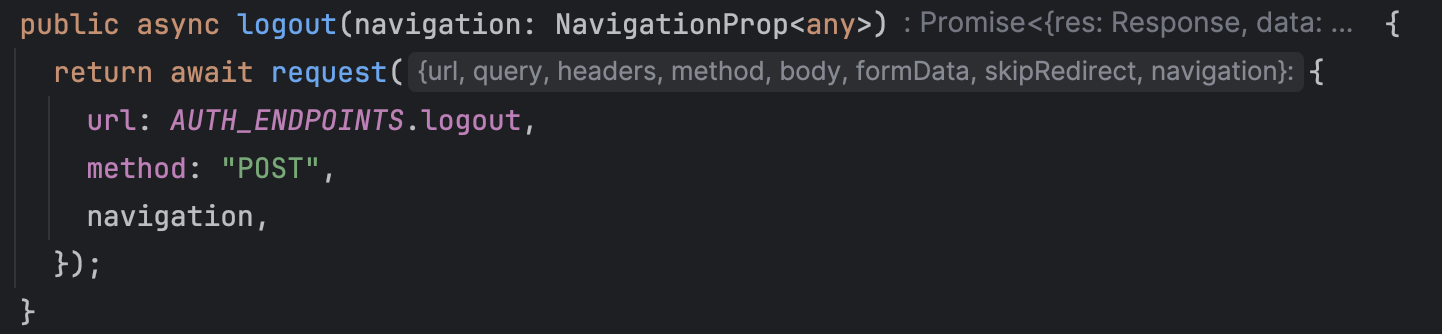
\includegraphics[width=0.7\textwidth]{chapters/chapter_8/screens/wylogowanie_mobile}
    \caption{Metoda “logout” zastosowana w aplikacji mobilnej.}
    \label{img:wylogowanie_mobile}
\end{figure}

\begin{figure}[H]
    \centering
    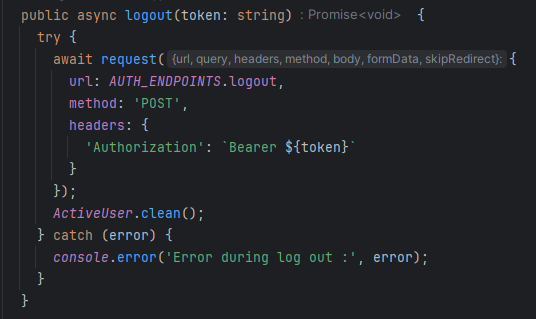
\includegraphics[width=0.7\textwidth]{chapters/chapter_8/screens/wylogowanie_web}
    \caption{Metoda “logout” zastosowana w aplikacji webowej.}
    \label{img:wylogowanie_web}
\end{figure}

Powyższe fragmenty serwisu odpowiadają za usunięcie danych użytkownika z pamięci lokalnej wykorzystujący endpoint dezaktywujący token autoryzacji.

\subsection{Edycja danych użytkownika}
Funkcjonalność umożliwiająca  edycję danych użytkownika.

\subsubsection{Backend}
Aplikacje frontendowe wysyłają dane do aktualizacji np. email. Jedynym obowiązkowym atrybutem przy aktualizacji jest \texttt{current\_password}. Po zweryfikowaniu zgodności hasła, system przystępuje do zmiany danych wprowadzonych przez użytkownika. Na koniec zostają zwrócone użytkownika z poprawionym polami.

\begin{figure}[H]
    \centering
    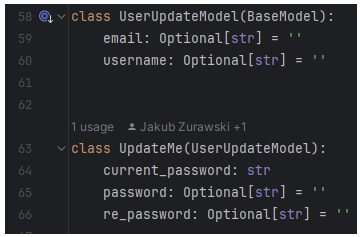
\includegraphics[width=0.5\textwidth]{chapters/chapter_8/screens/edit_user_backend_1}
    \caption{Implementacja klas modeli "UserUpdateModel" i "UpdateMe" w backendzie.}
    \label{img:edit_user_backend_1}
\end{figure}

\begin{figure}[H]
    \centering
    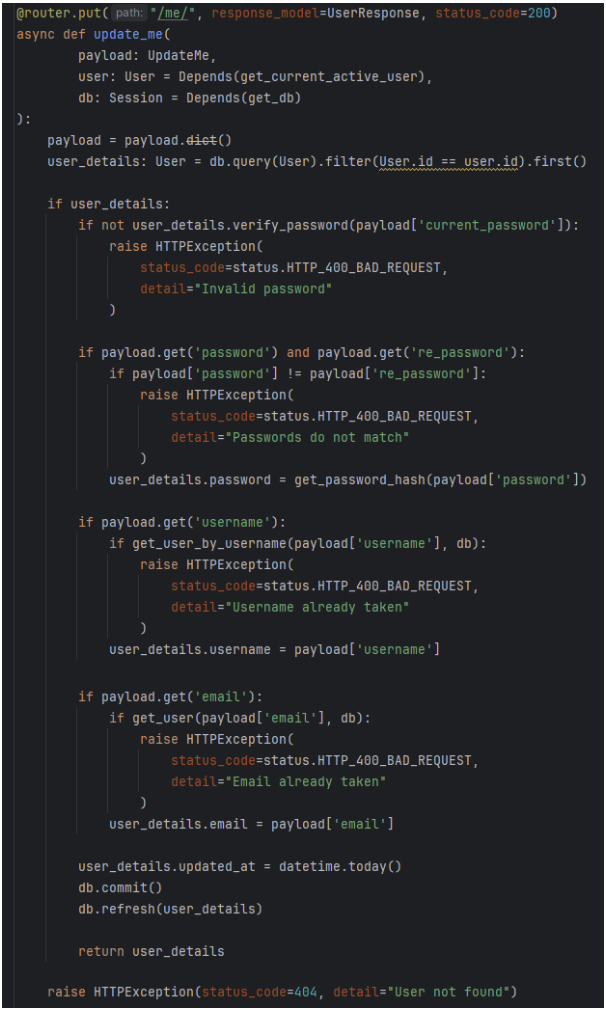
\includegraphics[width=0.7\textwidth]{chapters/chapter_8/screens/edit_user_backend_2}
    \caption{Implementacja kodu zmiany danych użytkownika w backendzie.}
    \label{img:edit_user_backend_2}
\end{figure}

\subsubsection{Aplikacja mobilna i aplikacja webowa}
W celu zmiany danych użytkownika, takich jak avatar, nickname, adres email czy hasło, użytkownik może skorzystać z odpowiednich formularzy dostępnych na stronie profilu użytkownika. Każda zmiana (za wyjątkiem zmiany avatara) wymaga uwierzytelnienia przez podanie aktualnego hasła. Poniżej opisane są poszczególne procesy.

\begin{figure}[H]
    \centering
    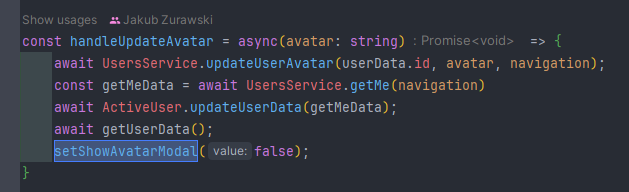
\includegraphics[width=0.7\textwidth]{chapters/chapter_8/screens/edit_user_mobile}
    \caption{Funkcja “handleAvatarSelect” zastosowany w aplikacji mobilnej.}
    \label{img:edit_user_mobile}
\end{figure}

\begin{figure}[H]
    \centering
    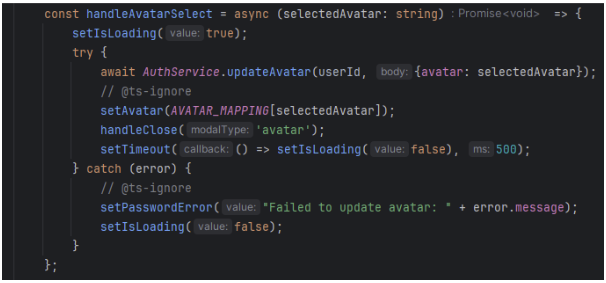
\includegraphics[width=0.7\textwidth]{chapters/chapter_8/screens/edit_user_web}
    \caption{Funkcja “handleAvatarSelect” zastosowany w aplikacji webowej.}
    \label{img:edit_user_web}
\end{figure}

\textbf{Zmiana avatara}\\
Aby zmienić avatar, użytkownik musi wybrać nowy avatar z dostępnych opcji. Po dokonaniu wyboru aplikacja wysyła żądanie do serwera w celu aktualizacji avatara. Po pomyślnej aktualizacji użytkownik zobaczy nowy avatar na stronie profilu oraz w widoku statystyk.\\


\textbf{Zmiana pseudonimu}\\
Aby zmienić pseudonim, użytkownik musi wprowadzić nowy pseudonim oraz aktualne hasło w odpowiednim formularzu. Po zatwierdzeniu formularza dane są walidowane:
\begin{itemize}
    \item Pseudonim musi zawierać 3-20 znaków i składać się wyłącznie z liter, cyfr lub podkreślników
    \item Aktualne hasło musi być poprawne
\end{itemize}
Jeśli dane są poprawne, aplikacja wysyła żądanie do serwera w celu aktualizacji pseudonimu. Po pomyślnej aktualizacji nowy pseudonim będzie wyświetlany na stronie profilu.\\


\textbf{Zmiana adresu email}\\
Aby zmienić adres email, użytkownik musi wprowadzić nowy adres email oraz aktualne hasło w odpowiednim formularzu. Po zatwierdzeniu formularza dane są walidowane:
\begin{itemize}
    \item Adres email musi mieć poprawny format
    \item Aktualne hasło musi być poprawne
\end{itemize}
Jeśli dane są poprawne, aplikacja wysyła żądanie do serwera w celu aktualizacji adresu email. Po pomyślnej aktualizacji użytkownik będzie logował się nowym adresem email.\\


\textbf{Zmiana hasła}\\
Aby zmienić hasło, użytkownik musi wprowadzić aktualne hasło, nowe hasło oraz potwierdzenie nowego hasła w odpowiednim formularzu. Po zatwierdzeniu formularza dane są walidowane:
\begin{itemize}
    \item Nowe hasło musi mieć co najmniej 8 znaków
    \item Potwierdzenie nowego hasła musi być zgodne z nowym hasłem
    \item Aktualne hasło musi być poprawne
\end{itemize}
Jeśli dane są poprawne, aplikacja wysyła żądanie do serwera w celu aktualizacji hasła.

\subsection{Usunięcie konta użytkownika}
Funkcjonalność umożliwiająca usunięcie konta użytkownika.

\subsubsection{Backend}
Aplikacje frontendowe wysyłają na api email użytkownika i hasło. Api sprawdza poprawność danych, następnie usuwa konto użytkownika.

\begin{figure}[H]
    \centering
    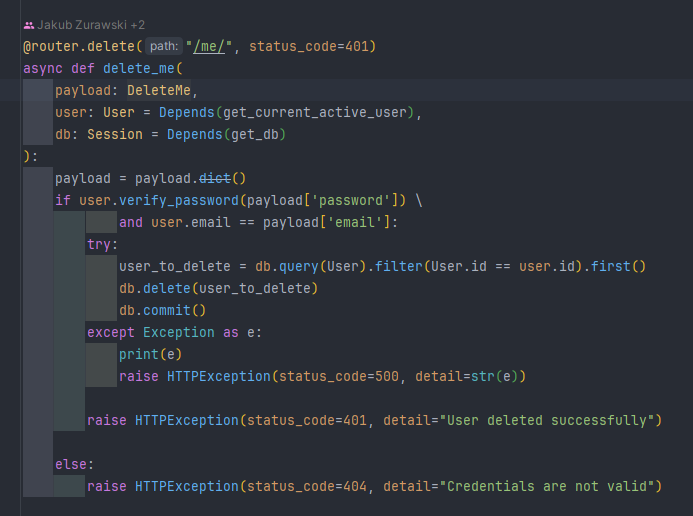
\includegraphics[width=0.7\textwidth]{chapters/chapter_8/screens/delete_user_backend}
    \caption{Implementacja kodu usunięcia użytkownika w backendzie.}
    \label{img:delete_user_backend}
\end{figure}

\subsubsection{Aplikacja moblina}
Użytkownik jest proszony o potwierdzenie czy aby na pewno chce usunąć konto. Po zatwierdzeniu zostaje przekierowany do formularza gdzie podaje email oraz hasło, które po zatwierdzeniu zostają wysłane na api.

\begin{figure}[H]
    \centering
    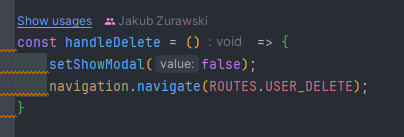
\includegraphics[width=0.7\textwidth]{chapters/chapter_8/screens/delete_user_mobile_1}
    \caption{Wywołanie funkcji “handleDelete” zastosowanego w aplikacji mobilnej.}
    \label{img:delete_user_mobile_1}
\end{figure}

\begin{figure}[H]
    \centering
    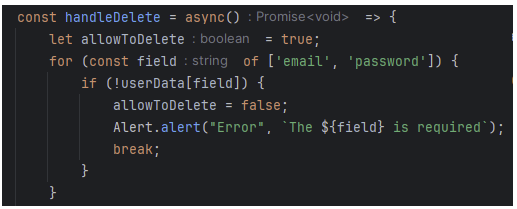
\includegraphics[width=0.7\textwidth]{chapters/chapter_8/screens/delete_user_mobile_2}
    \caption{Funkcja “handleDelete” zastosowany w aplikacji mobilnej.}
    \label{img:delete_user_mobile_2}
\end{figure}

\subsubsection{Aplikacja webowa}

Jeżeli po potwierdzeniu wyboru prawidłowym hasłem, funkcja wykryje error 401 (Unauthorized), oznaczać to będzie że konto zostało usunięte. Następnie pojawia się komunikat o usunięciu który przekierowuje do strony logowania

\begin{figure}[H]
    \centering
    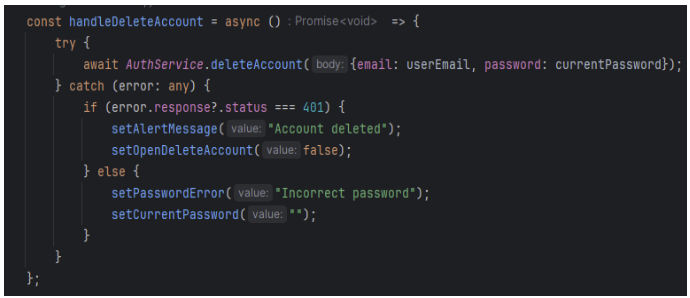
\includegraphics[width=0.7\textwidth]{chapters/chapter_8/screens/delete_user_web}
    \caption{Funkcja “handleDelete” zastosowany w aplikacji webowej.}
    \label{img:delete_user_web}
\end{figure}

\subsection{Tworzenie talii fiszek}

Funkcjonalność umożliwiająca tworzenie talii fiszek.

\subsubsection{Backend}

Utworzono metodę post, która umożliwia tworzenie talii o podanej nazwie i kategorii. Do tworzenia fiszki używana jest osobna metoda post, która przyjmuje treść dla przedniej i tylnej strony karty, a także id talii do, której utworzona fiszka zostanie przypisana.

\begin{figure}[H]
    \centering
    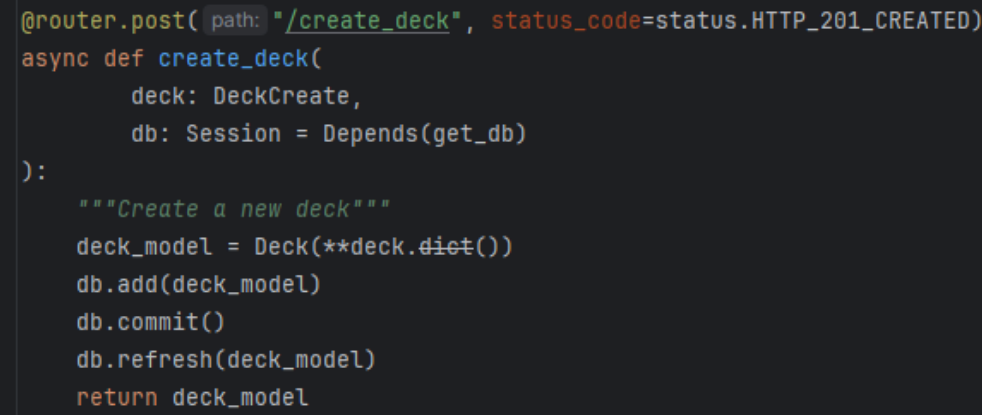
\includegraphics[width=0.7\textwidth]{chapters/chapter_8/screens/create_deck_backend}
    \caption{Logika tworzenia decku po stronie serwera.}
    \label{img:create_deck_backend}
\end{figure}

\begin{figure}[H]
    \centering
    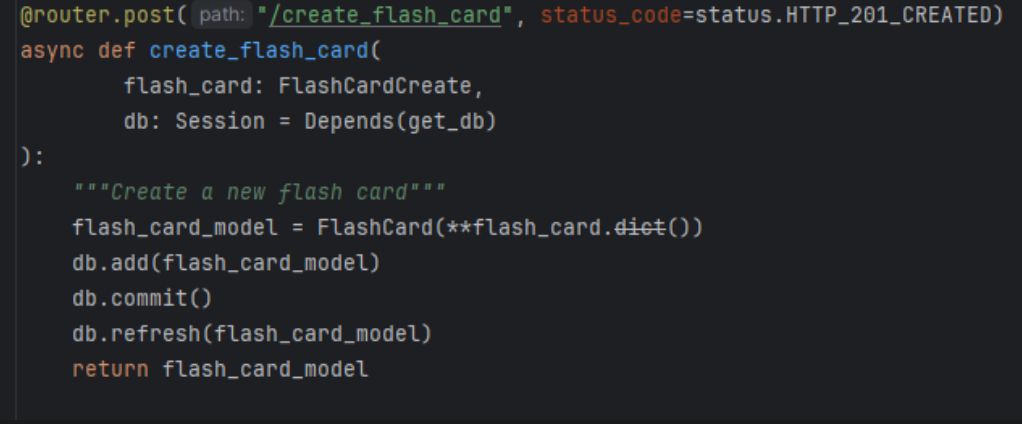
\includegraphics[width=0.7\textwidth]{chapters/chapter_8/screens/create_flash_card_backend}
    \caption{Logika tworzenia fiszek po stronie serwera.}
    \label{img:create_flash_card_backend}
\end{figure}

\subsubsection{Aplikacja mobilna}
Dodanie fiszki jest możliwe po przejściu do widoku jej tworzenia z podglądu wybranej talii. Wymagane jest uzupełnienie pól przedniej i tylnej strony fiszki. Tworzenie odbywa się przez wysłanie danych do odpowiedniego endpointu.

\begin{figure}[H]
    \centering
    \includegraphics[width=0.7\textwidth]{chapters/chapter_8/screens/create_deck_mobile}
    \caption{Funkcja obsługująca tworzenie nowej fiszki..}
    \label{img:create_deck_mobile}
\end{figure}

\subsubsection{Aplikacja webowa}

Użytkownik aby utworzyć talię musi wypełnić pole tekstowe dla nazwy i kategorii talii, następnie musi uzupełnić treść dla przedniej i tylnej strony fiszki. Po kliknięciu create deck dane z formularzy zostają przekazane do funkcji, która zebrane dane przekazuje do serwisu odpowiedzialnego za komunikację z endpointem do tworzenia talii i endpointem do tworzenia fiszki.

\begin{figure}[H]
    \centering
    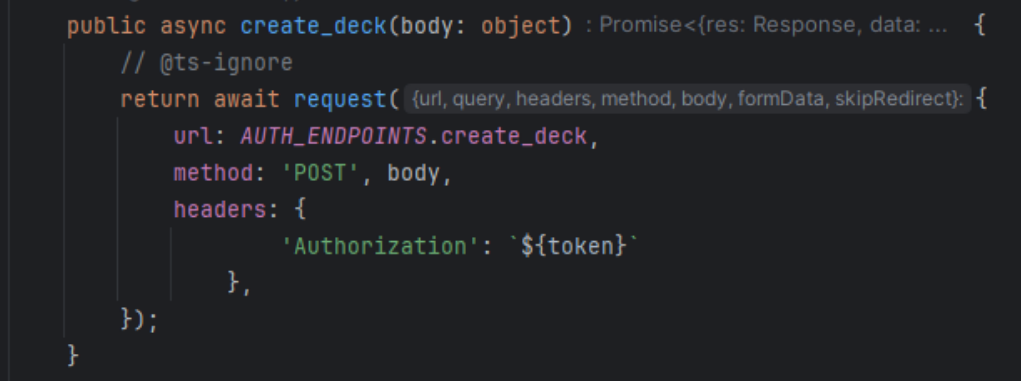
\includegraphics[width=0.7\textwidth]{chapters/chapter_8/screens/create_deck_web}
    \caption{Funkcja serwisu odpowiedzialna za komunikację z endpointem do tworzenia decku.}
    \label{img:create_deck_web}
\end{figure}

\begin{figure}[H]
    \centering
    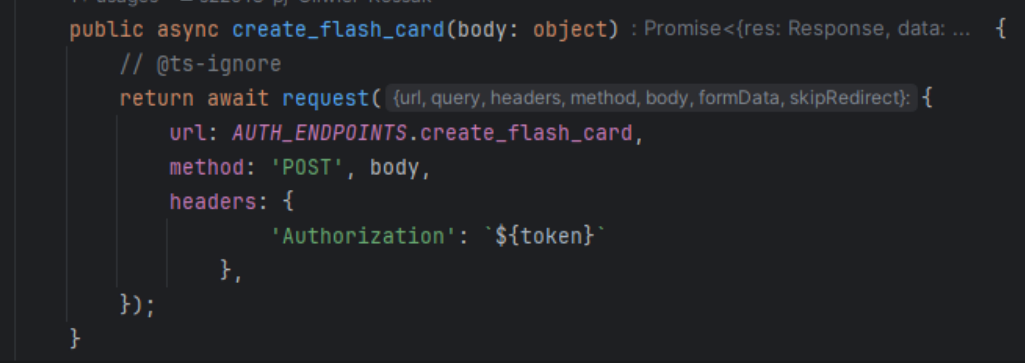
\includegraphics[width=0.7\textwidth]{chapters/chapter_8/screens/create_flash_card_web}
    \caption{Funkcja serwisu odpowiedzialna za komunikację z endpointem do tworzenia fiszki.}
    \label{img:create_flash_card_web}
\end{figure}

\subsection{Usunięcie talii fiszek}

Funkcjonalność umożliwiająca usunięcie talii fiszek.

\subsubsection{Backend}

Został utworzony endpoint \texttt{delete_deck}, która pozwala na usunięcie talii o podanym id wraz z wszystkimi powiązanymi fiszkami.

\begin{figure}[H]
    \centering
    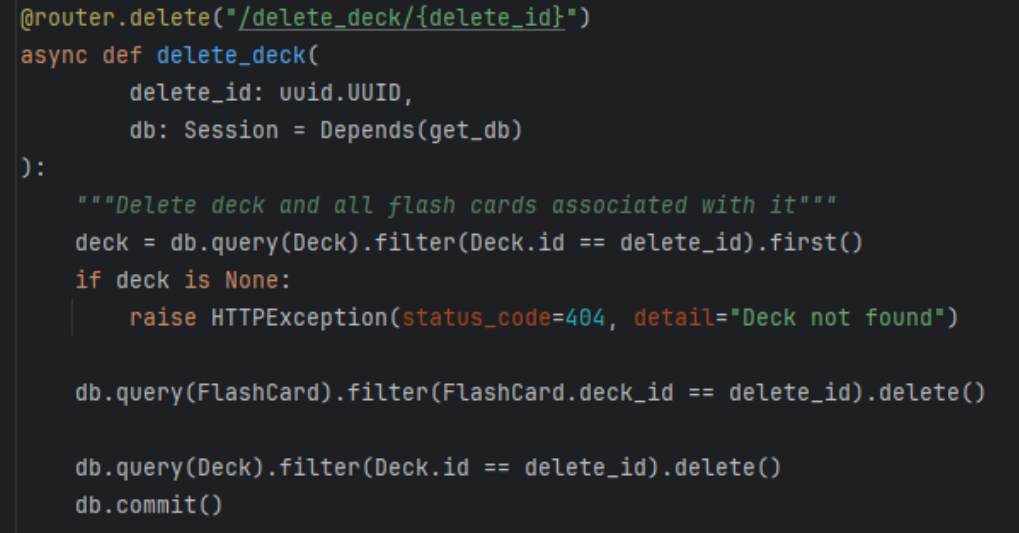
\includegraphics[width=0.7\textwidth]{chapters/chapter_8/screens/delete_deck_backend}
    \caption{Logika usuwająca talie i wszystkie należące do niej fiszki.}
    \label{img:delete_deck_backend}
\end{figure}


\subsubsection{Aplikacja moblina}
Usunięcie talii jest możliwe z poziomu jej opcji. Po wybraniu tej opcji do api zostaje wysłane zapytanie o usunięcie talii. W zapytaniu przekazywane jest id decku.

\begin{figure}[H]
    \centering
    \includegraphics[width=0.7\textwidth]{chapters/chapter_8/screens/delete_deck_mobile}
    \caption{Funkcja odpowiedzialna za obsługę usunięcia decku.}
    \label{img:delete_deck_mobile}
\end{figure}

\subsubsection{Aplikacja webowa}

Użytkownik aby usunąć talię klika w opcje, następnie wybiera delete deck. Po kliknięciu id aktualnej talii zostaje pobrane z pamięci lokalnej i przekazane do serwisu, który łączy się z bakcendowym endpoint em do usuwania talii. Endpoint usuwa z bazy danych talię o podanym id i wszystkie należące do niego fiszki.

\begin{figure}[H]
    \centering
    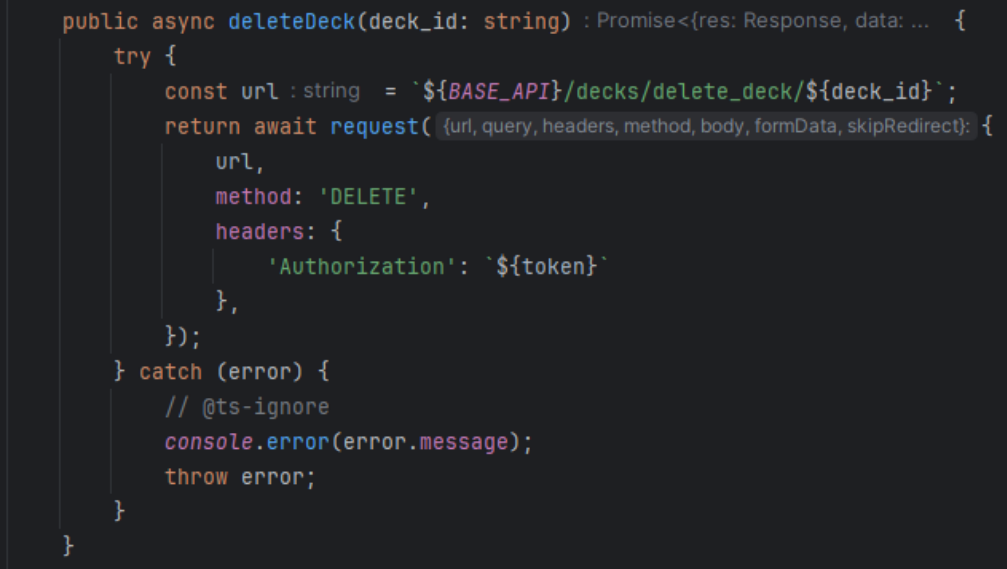
\includegraphics[width=0.7\textwidth]{chapters/chapter_8/screens/delete_deck_web}
    \caption{Funkcja serwisu odpowiedzialna za komunikację z endpointem do usuwania decku.}
    \label{img:delete_deck_web}
\end{figure}

\subsection{Edycja talii fiszek}

Funkcjonalność umożliwiająca aktualizowanie zawartości talii fiszek.

\subsubsection{Backend}

Zostały utworzone metody put, pozwalające na komunikację z bazą danych w celu aktualizacji informacji o fiszkach i taliach.

\begin{figure}[H]
    \centering
    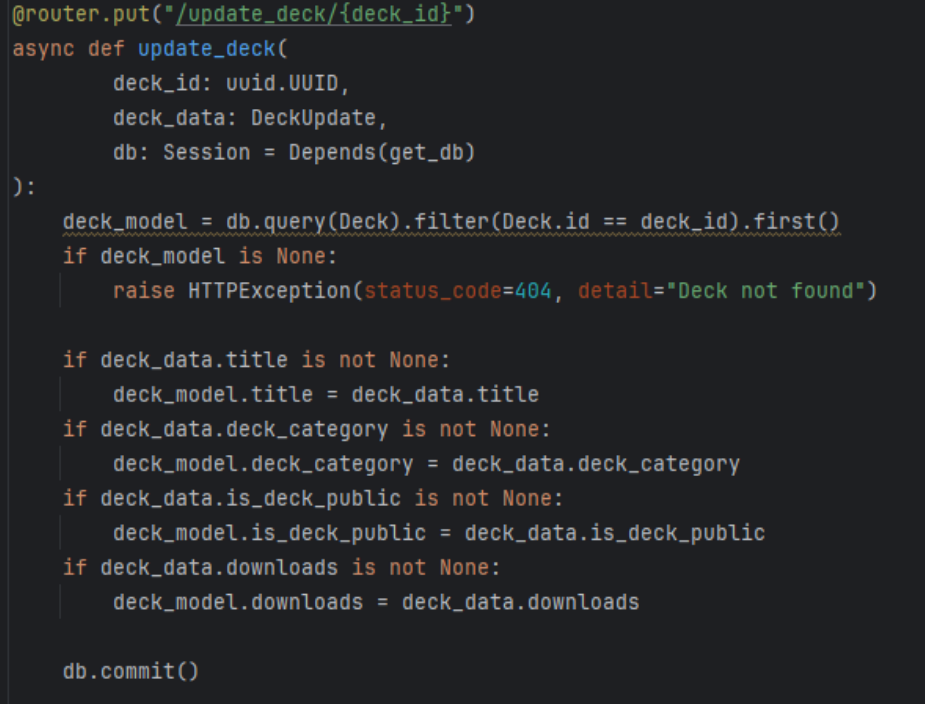
\includegraphics[width=0.7\textwidth]{chapters/chapter_8/screens/update_deck_backend}
    \caption{Endpoint odpowiedzialny za aktualizację danych talii o podanym id}
    \label{img:update_deck_backend}
\end{figure}

\begin{figure}[H]
    \centering
    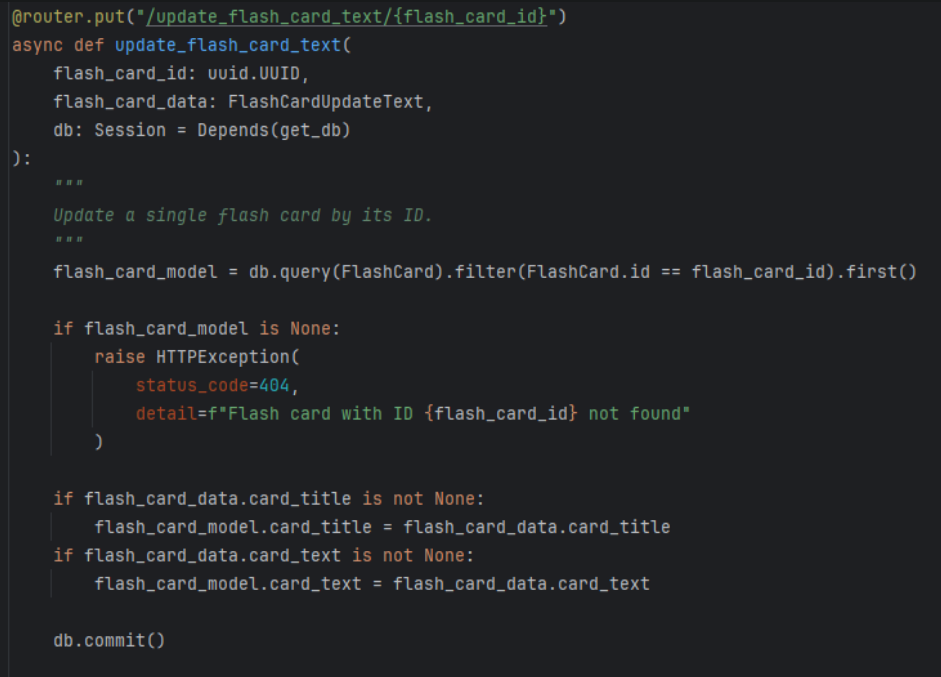
\includegraphics[width=0.7\textwidth]{chapters/chapter_8/screens/update_flash_card_text_backend}
    \caption{Endpoint odpowiedzialny za aktualizację danych fiszki o podanym id}
    \label{img:update_flash_card_backend}
\end{figure}

% TODO daniel
\subsubsection{Aplikacja moblina}
\subsubsection{Aplikacja webowa}

Użytkownik w celu zmiany nazwy talii lub kategorii musi otworzyć okno opcji następnie klika w przycisk zmiany danych. Po wykonanie tych operacji pojawia się formularz do zmiany nazwy talii i kategorii. Użytkownik może podać nowe dane i kliknąć przycisk accept. Nowe dane zostają przekazane do funkcji zmiany nazwy i kategorii następnie przechwycone dane zostają przekazane do serwisu, który łączy się z backendowym endpointem. Następnie endpoint łączy się z bazą danych w celu aktualizacji talii o otrzymane dane. Tak samo wygląda proces aktualizacji danych fiszki, po kliknięciu w ołówek znajdujący się na fiszce pojawia się formularz do aktualizacji danych fiszki.

\begin{figure}[H]
    \centering
    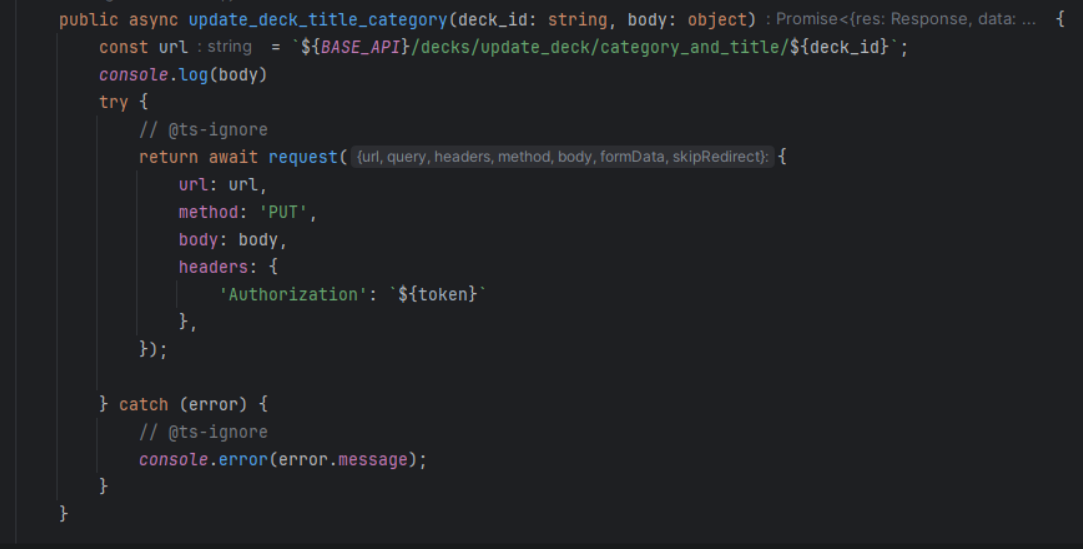
\includegraphics[width=0.7\textwidth]{chapters/chapter_8/screens/update_deck_web}
    \caption{Service służący do komunikacji z backendowym endpointem do aktualizacji danych talii}
    \label{img:update_deck_web}
\end{figure}

\begin{figure}[H]
    \centering
    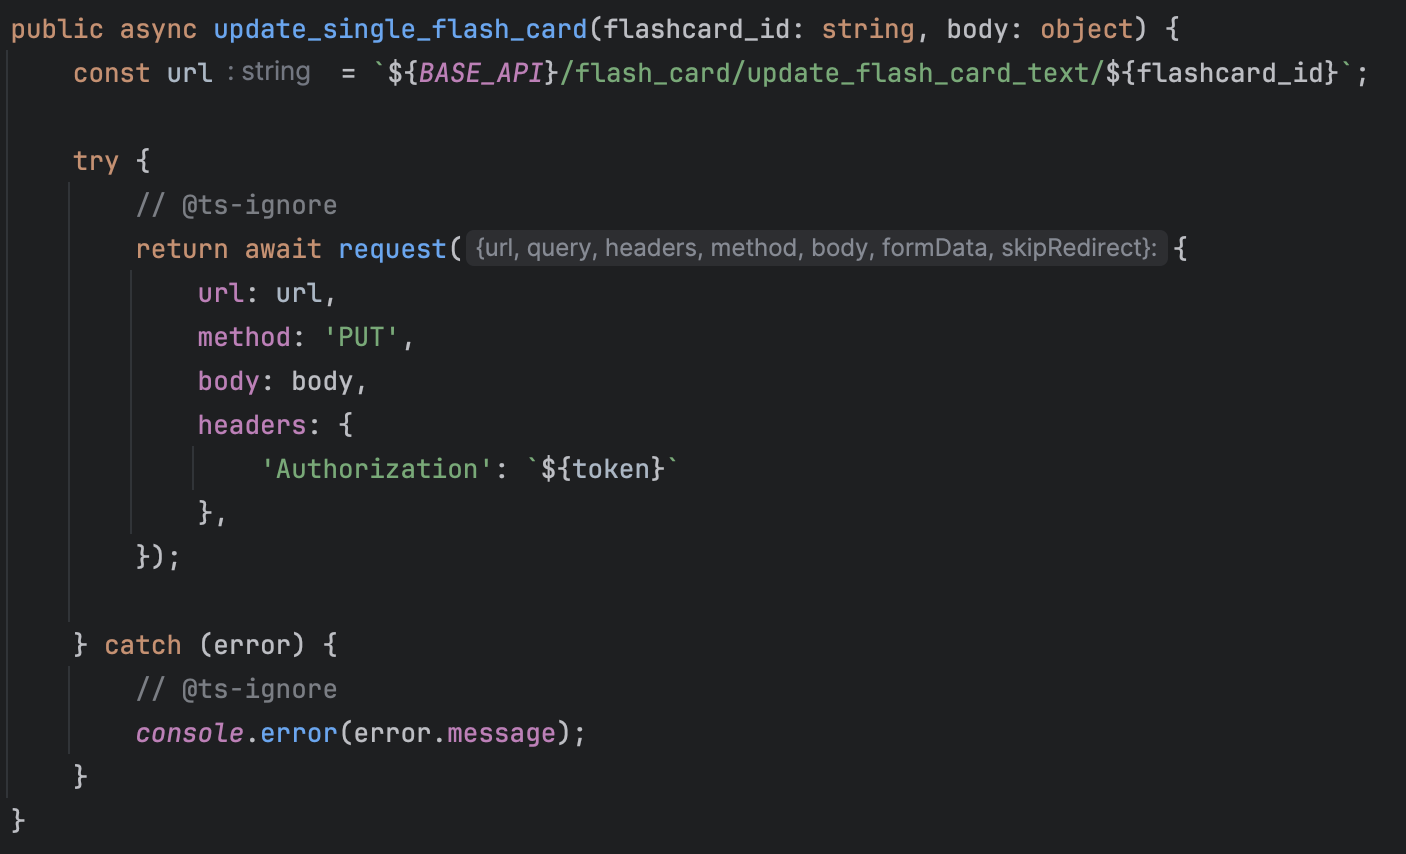
\includegraphics[width=0.7\textwidth]{chapters/chapter_8/screens/update_flash_card_text_web}
    \caption{Service służący do komunikacji z backendowym endpointem do aktualizacji danych fiszki}
    \label{img:update_flash_card_web}
\end{figure}

\subsection{Tryb uczenia się z talii fiszek}

\subsubsection{Backend}

Model fiszki zawiera kolumnę \texttt{is_memorized}, która przy tworzeniu fiszki jest domyślnie ustawiona na false, wartość ta oznacza, że użytkownika jeszcze nie nauczył się danej treści fiszki. Jeżeli użytkownik uzna, że fiszka została przez niego zapamiętana, to wartość kolumny \texttt{is_memorized} po zakończonym uczeniu się zostanie zaktualizowana na wartość true. Do aktualizacji danych fiszek została wykorzystany endpoint, który przyjmuje listę fiszek i następnie aktualizuje dane wszystkich fiszek zawartych w przesłanej liście.

\begin{figure}[H]
    \centering
    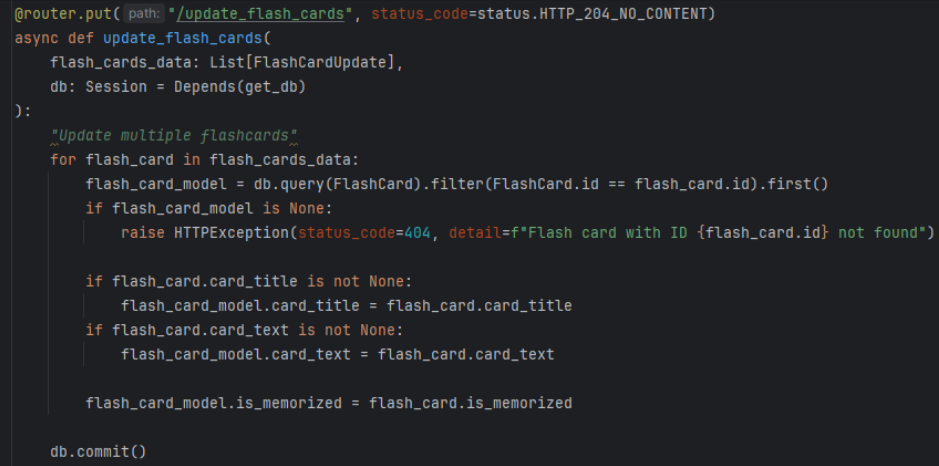
\includegraphics[width=0.7\textwidth]{chapters/chapter_8/screens/update_flash_card_memorized_backend}
    \caption{Logika aktualizacji przesłanych fiszek}
    \label{img:update_flash_card_memorized_backend}
\end{figure}

\subsubsection{Aplikacja moblina}

Po wejściu na widok nauki, aplikacja ściąga fiszki użytkownika. W trakcie nauki użytkownik może wybrać dwie opcje remember lub not remember. W momencie kliknięcia przycisku remember informacje o fiszce zostaną dodane do listy nauczonych fiszek, które potem zostaną zaktualizowane w bazie. Po zakończeniu trybu nauki, aplikacja ściąga na nowo listę fiszek i filtruje je po polu ‘\texttt{is_memorized} ‘. Fiszki które mają ustawione \texttt{is_memorized} na true, nie zostaną ponownie wyświetlone w trybie nauki.

\begin{figure}[H]
    \centering
    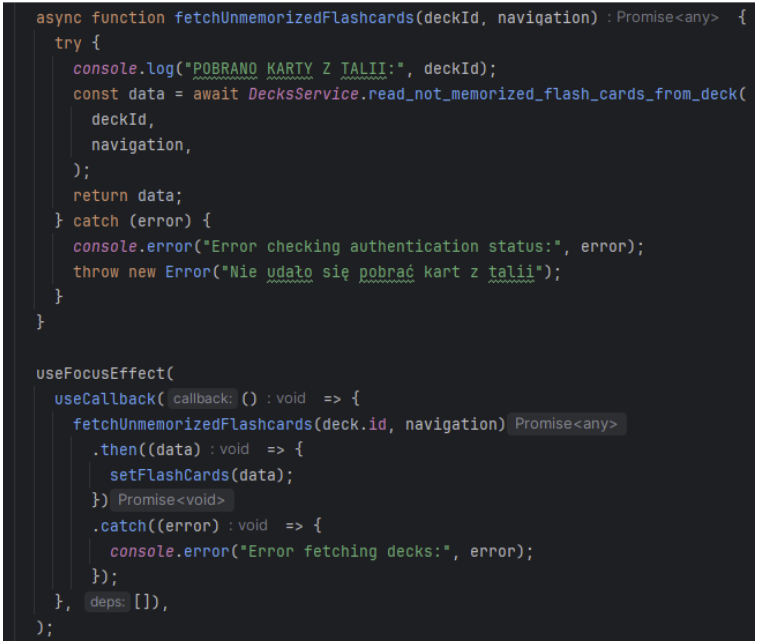
\includegraphics[width=0.7\textwidth]{chapters/chapter_8/screens/get_unmemorized_flash_cards_mobile}
    \caption{Funkcja ściągająca niezapamiętane fiszki}
    \label{img:get_unmemorized_flash_cards_mobile}
\end{figure}

\begin{figure}[H]
    \centering
    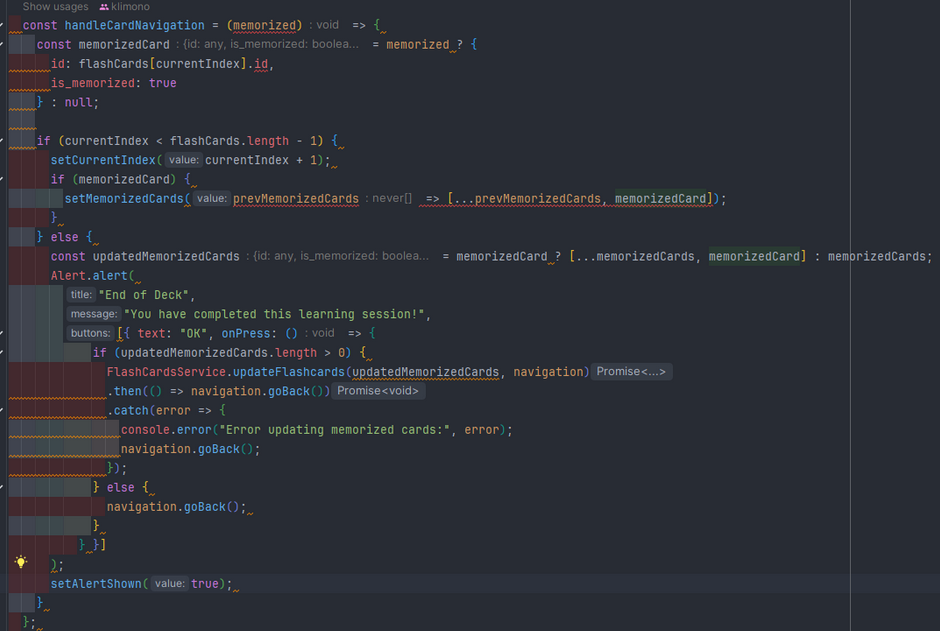
\includegraphics[width=0.7\textwidth]{chapters/chapter_8/screens/update_unmemorized_flash_cards_mobile}
    \caption{Funkcja aktualizacji zapamiętanych fiszek}
    \label{img:update_unmemorized_flash_cards_mobile}
\end{figure}

\subsubsection{Aplikacja webowe}

Po uruchomieniu trybu uczenia użytkownik widząc fiszkę może kliknąć przycisk remember lub not remember. W przypadku kliknięcia przycisku remember informacje o fiszce zostaną dodane do listy fiszek, które zostaną zaktualizowane. Po zakończeniu trybu uczenia list z fiszkami, które zostały oznaczone jako zapamiętane zostaje przekazana do serwisuje, który następnie przekazuje dane do bakcendowego endpointu w celu aktualizacji danych fiszek w bazie danych. Kolumna \texttt{is_memorized} wszystkich przekazanych fiszek zostaje ustawiona na wartość true. Fiszki, których kolumna \texttt{is_memorized} jest ustawiona na true nie wyświetlają się w trybie uczenia.

\begin{figure}[H]
    \centering
    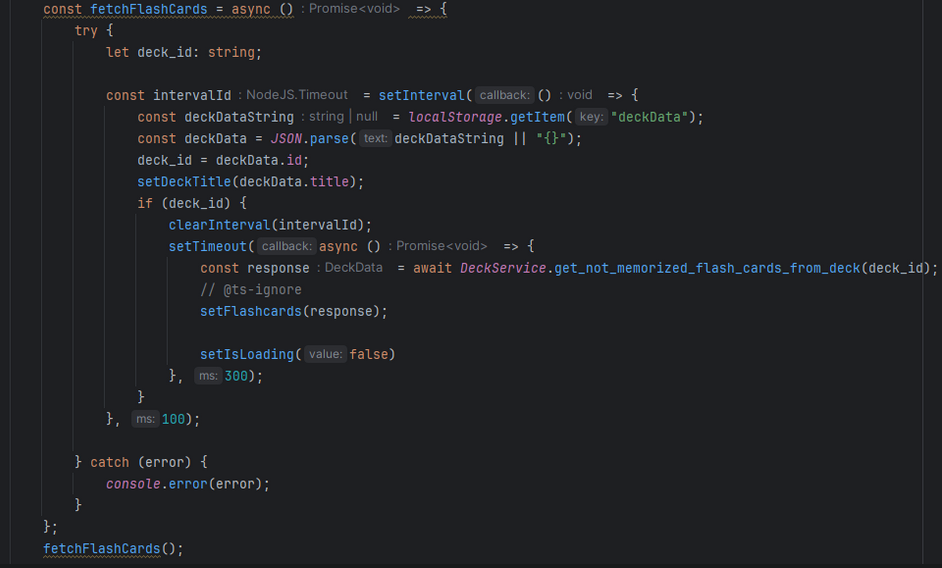
\includegraphics[width=0.7\textwidth]{chapters/chapter_8/screens/get_unmemorized_flash_cards_web}
    \caption{Funkcja ściągająca niezapamiętane fiszki}
    \label{img:get_unmemorized_flash_cards_web}
\end{figure}

\begin{figure}[H]
    \centering
    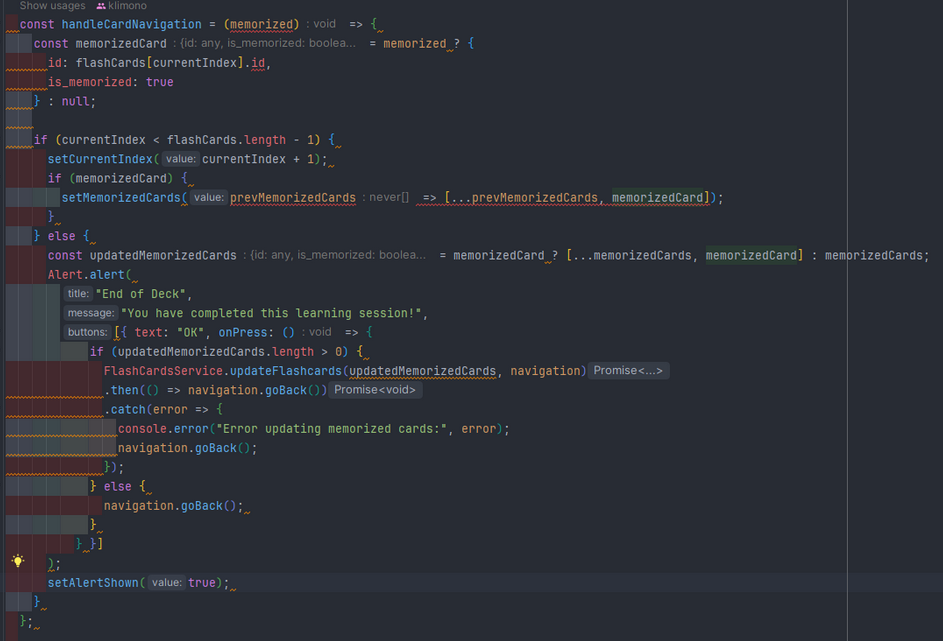
\includegraphics[width=0.7\textwidth]{chapters/chapter_8/screens/pass_unmemorized_flash_cards_web}
    \caption{Funkcja aktualizacji zapamiętanych fiszek}
    \label{img:pass_unmemorized_flash_cards_web}
\end{figure}

\begin{figure}[H]
    \centering
    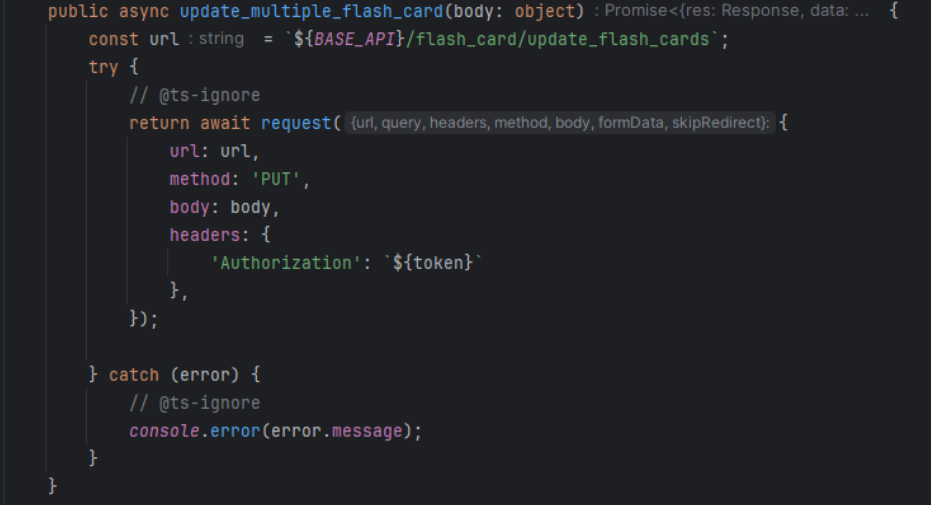
\includegraphics[width=0.7\textwidth]{chapters/chapter_8/screens/update_unmemorized_flash_cards_web}
    \caption{Funkcja aktualizacji zapamiętanych fiszek}
    \label{img:update_unmemorized_flash_cards_web}
\end{figure}